A three-dimensional elastic computer model of the substructure is analyzed using XC. The model includes first floor frame and columns (see figure \ref{model}). The hollow core planks ar modelled using shell elements, while beams and columns are modelled using frame elements. Loads transmited by 2$^{nd}$, 3$^{rd}$ floors and roof are applied to the 1$^{st}$. Load layout is shown in figure \ref{loadLay}. See in figures \ref{LC_D} to \ref{LC_W_NS} load distribution for each load case.

Linear loads are expressed in $\mathrm{kN/m}$ and surface loads in $\mathrm{kN/m^2}$, where:
\begin{center}
  \begin{tabular}{ll}
    1 $\mathrm{kN/m}$ = & 68.52178 lb/ft \\
    1 $\mathrm{kN/m^2}$ = & 20.885434 psf \\
  \end{tabular}
  \end{center}

\begin{Figure}
    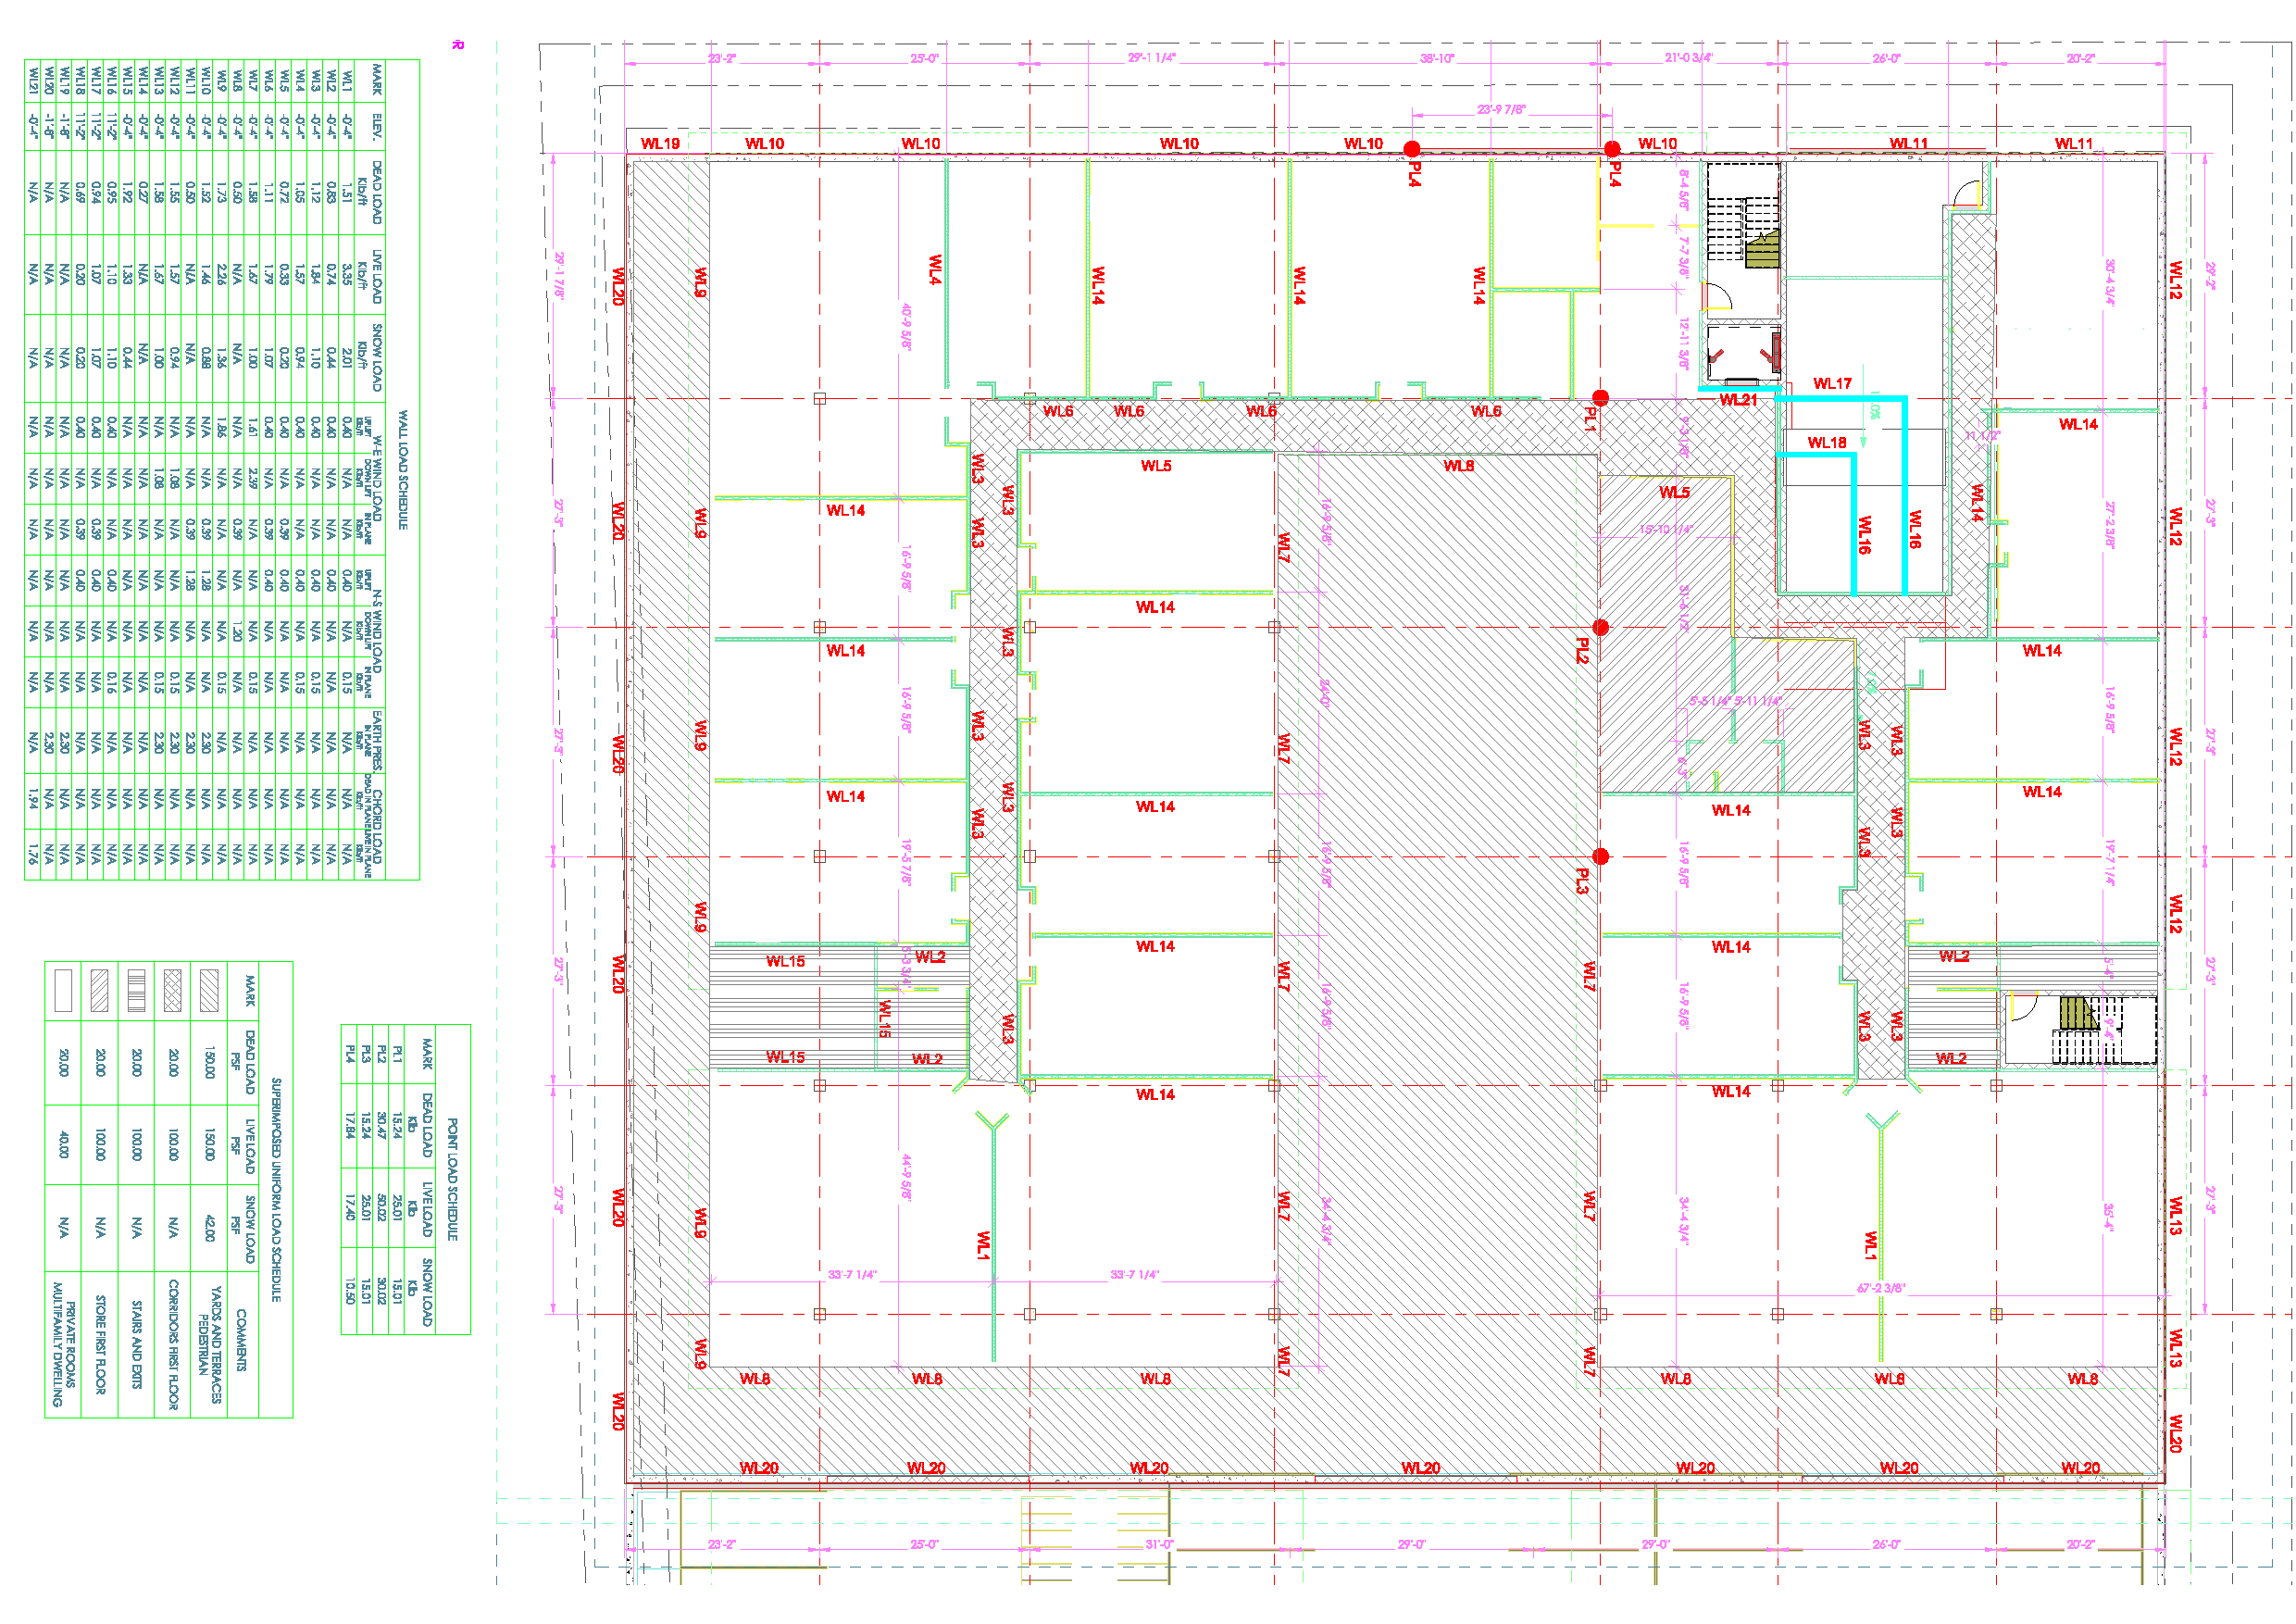
\includegraphics[width=150mm]{figures/loads_layout}
    \captionof{figure}{Load layout on first floor.}
    \label{loadLay}
\end{Figure}



\captionsetup[figure]{font=footnotesize}
\twocolumn
\begin{Figure}
    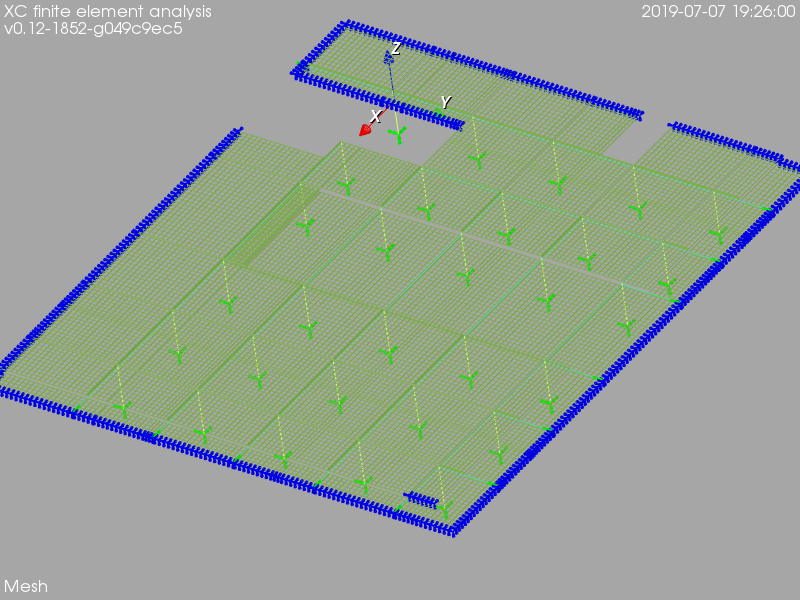
\includegraphics[width=\linewidth]{figures/mesh}
    \captionof{figure}{Elastic model, mesh.}
    \label{model}
\end{Figure}
\begin{Figure}
    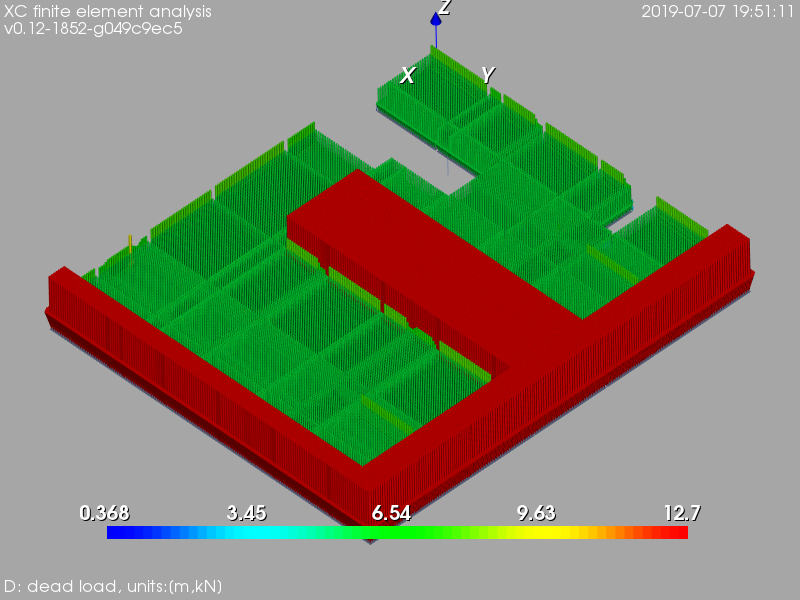
\includegraphics[width=\linewidth]{figures/LC_D}
    \captionof{figure}{Load case D: dead load (include slab selfweight) [units: kN,m].}
    \label{LC_D}
\end{Figure}

\begin{Figure}
    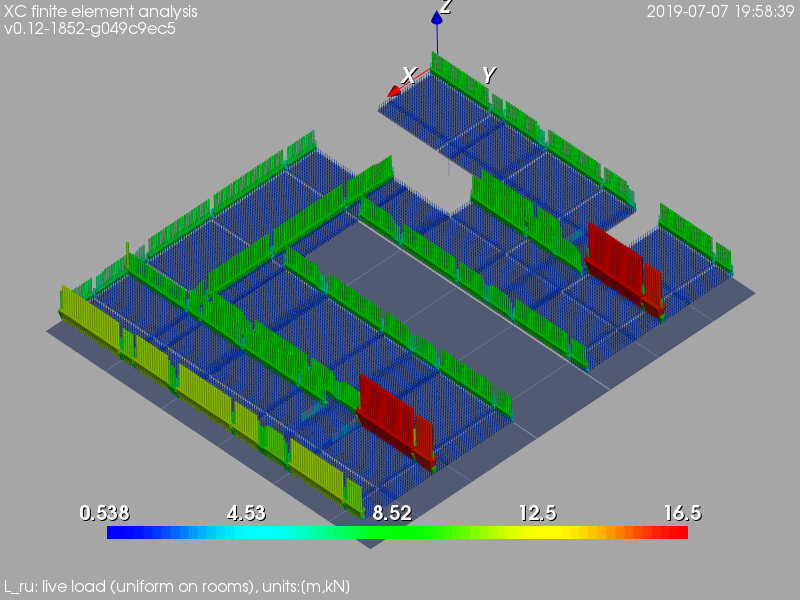
\includegraphics[width=\linewidth]{figures/LC_L_ru}
    \captionof{figure}{Load case Lru: live load (uniform on rooms) [units: kN,m].}
    \label{LC_L_ru}
\end{Figure}

\begin{Figure}
    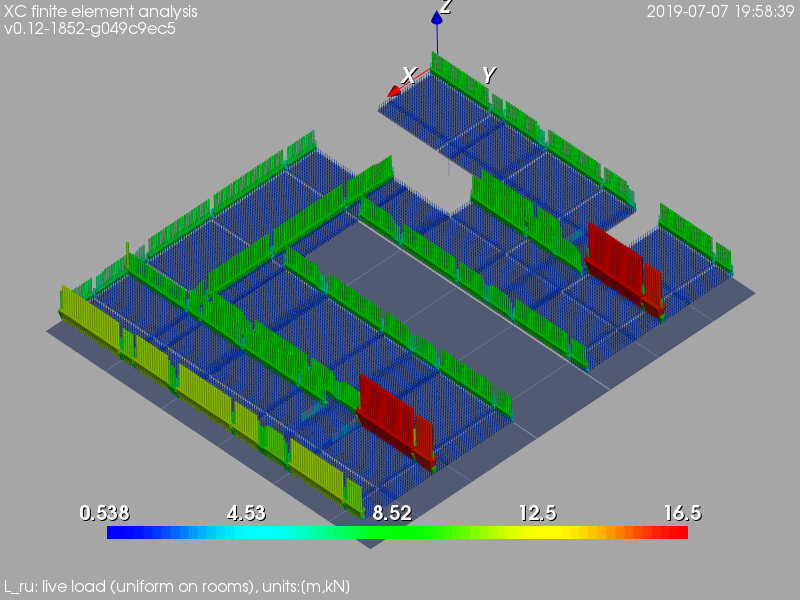
\includegraphics[width=\linewidth]{figures/LC_L_rs}
    \captionof{figure}{Load case Lrs:  live load (staggered pattern on rooms) [units: kN,m].}
    \label{LC_L_rs}
\end{Figure}

\begin{Figure}
    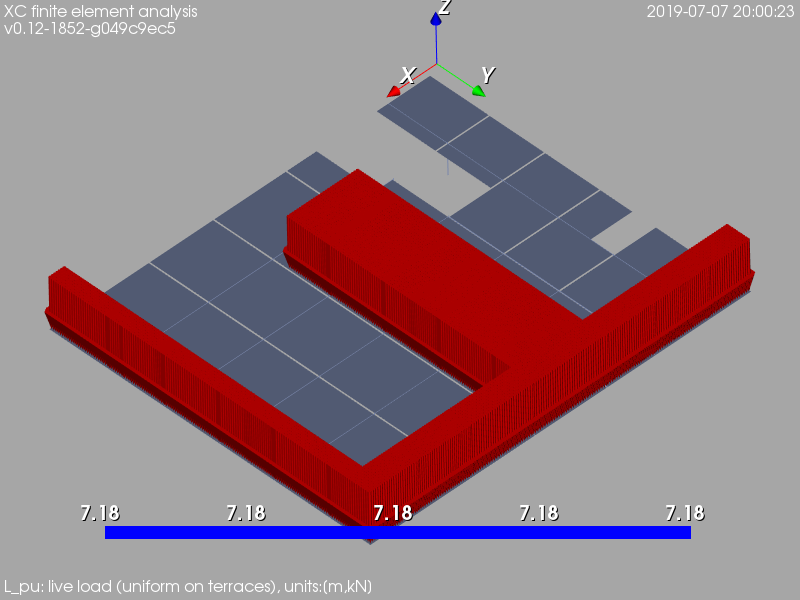
\includegraphics[width=\linewidth]{figures/LC_L_pu}
    \captionof{figure}{Load case Lpu: live load (uniform on patios) [units: kN,m].}
    \label{LC_L_pu}
\end{Figure}

\begin{Figure}
    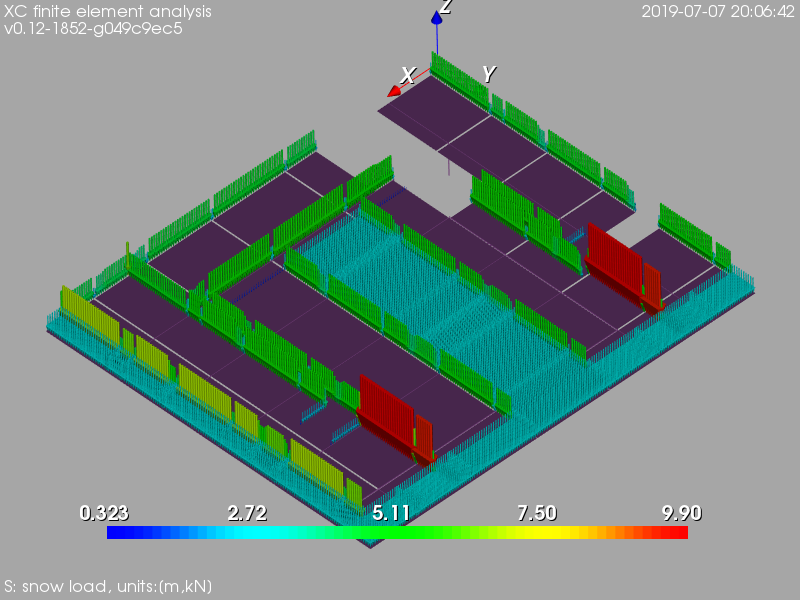
\includegraphics[width=\linewidth]{figures/LC_S}
    \captionof{figure}{Load case S: snow [units: kN,m].}
    \label{LC_S}
\end{Figure}
\begin{Figure}
    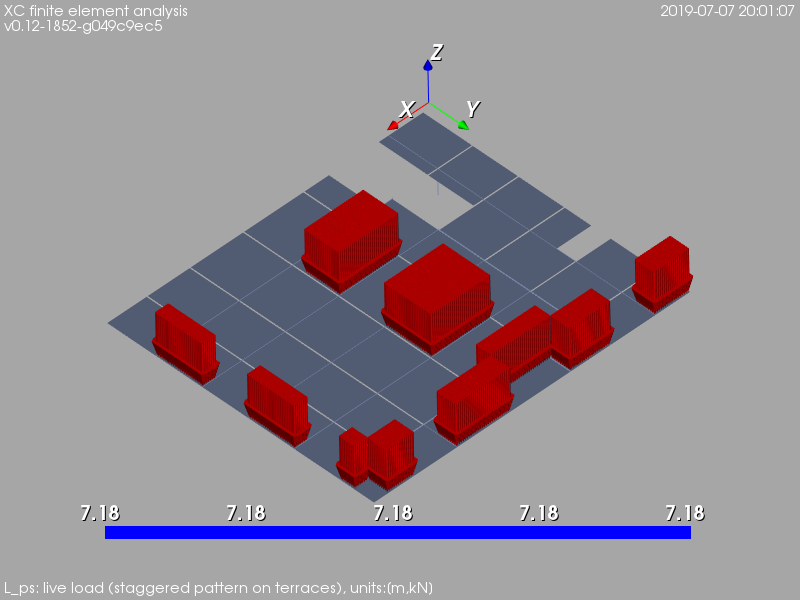
\includegraphics[width=\linewidth]{figures/LC_L_ps}
    \captionof{figure}{Load case Lps:  live load (staggered pattern on patios) [units: kN,m].}
    \label{LC_L_ps}
\end{Figure}

\begin{Figure}
    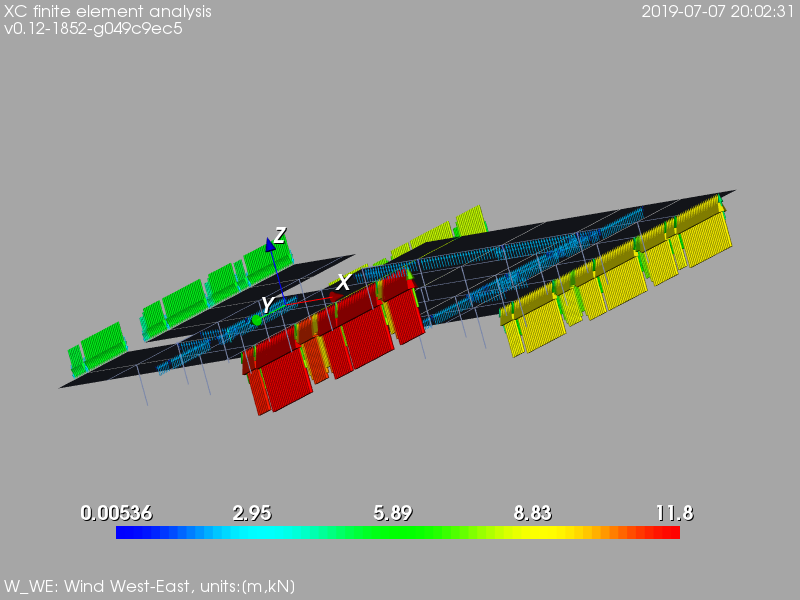
\includegraphics[width=\linewidth]{figures/LC_W_WE}
    \captionof{figure}{Load case W\_WE:  wind West-East [units: kN,m].}
    \label{LC_W_WE}
\end{Figure}

\begin{Figure}
    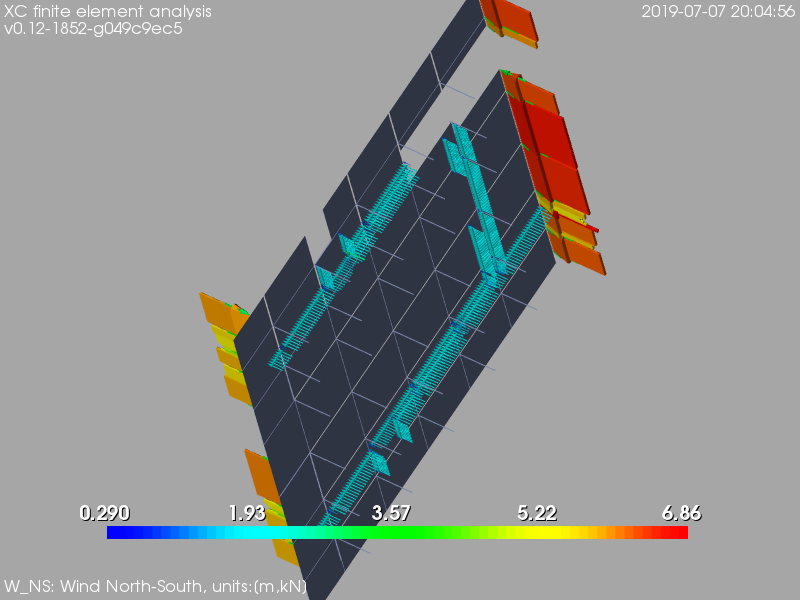
\includegraphics[width=\linewidth]{figures/LC_W_NS}
    \captionof{figure}{Load case W\_NS: wind North-South [units: kN,m].}
    \label{LC_W_NS}
\end{Figure}
\onecolumn
